\section{Introduction}\label{sec:introduction}

\begin{figure*}[t]
  \centering
  
\includegraphics[width=\textwidth]{fig_1_composite.pdf}
  \caption{Overview of IRT person-fit detection. (a)~A clean model's responses track the IRT-predicted probability curve; (b)~a contaminated model shows anomalous successes on hard items (red diamonds), producing a large $|\Delta\ell_z^*|$. (c)~Effect-size landscape: baseline accuracy vs.\ Cohen's $|d|$ across model families (diamonds: 5\%, triangles: 15\%, squares: 25\%, circles: 50\%; multi-seed means where available, single-seed otherwise; values from Table~\ref{tab:cohens_d}). (d)~Dose-response trajectories; free-$\theta$ shows non-monotonic artifact, fixed-$\theta$ recovers consistent positive dose-response.}
  \label{fig:composite}
\end{figure*}

\begin{figure*}[t]
  \centering
  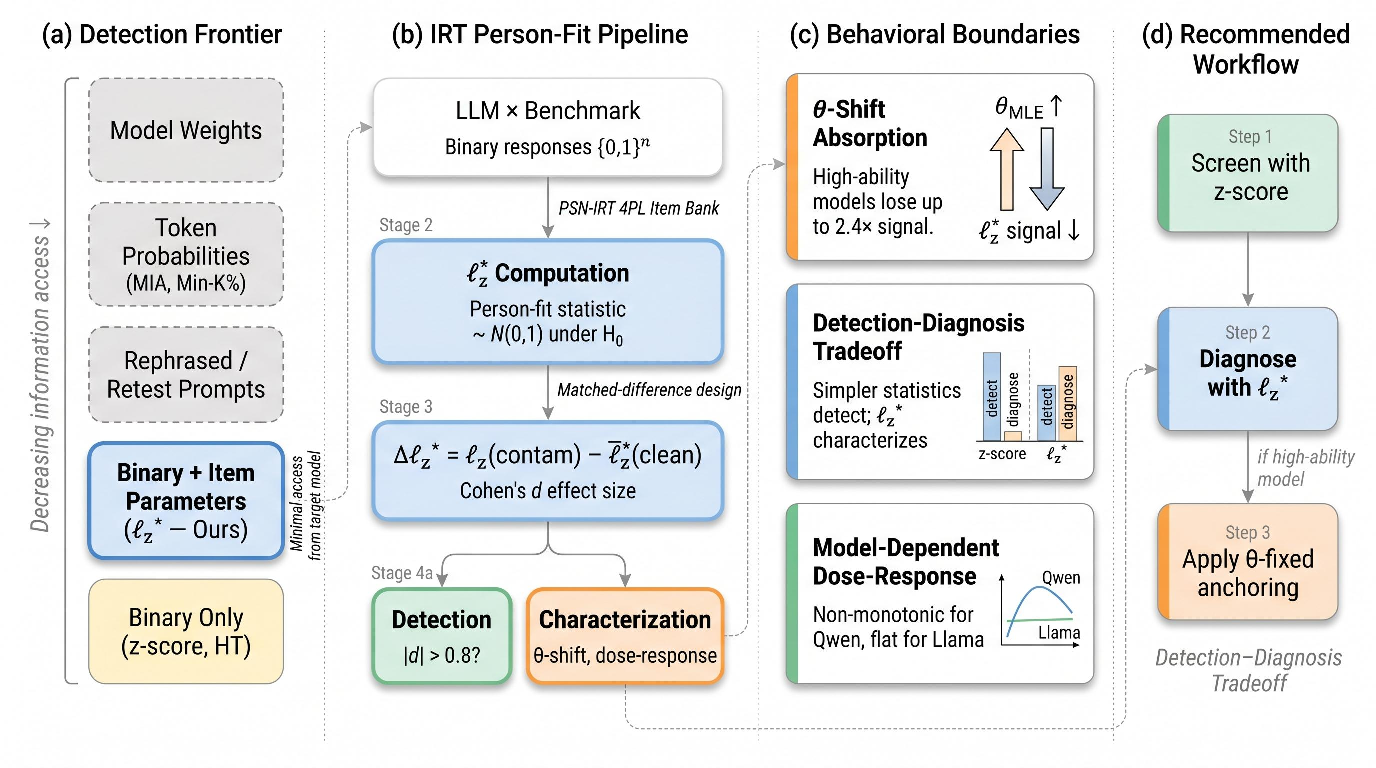
\includegraphics[width=\textwidth]{fig_framework.pdf}
  \caption{Overview of \irtfit{}: (a)~positioning in the detection frontier by information access; (b)~pipeline from binary responses through $\ell_z^*$ person-fit analysis to detection and characterization; (c)~three behavioral boundaries discovered; (d)~recommended practitioner workflow.}
  \label{fig:pipeline}
\end{figure*}

Benchmark contamination (the unintended inclusion of evaluation data in training corpora) poses a growing threat to LLM evaluation integrity \citep{dodge2021, magar2022, sainz2023}, as the probability of overlap increases structurally with expanding corpora and benchmarks \citep{jacovi2023, chang2024survey}.
Existing detection methods all require privileged access beyond binary response records: training corpora, token-level probabilities, crafted prompts, or multiple test variants (\S\ref{sec:related_work}).
Moreover, all log-probability-based detectors fail after RL post-training \citep{wang2025fragility}, motivating the question: \emph{what can binary response patterns alone reveal about contamination?}

A contaminated LLM is functionally analogous to a test-taker with item preknowledge: both produce response patterns where difficult items are answered correctly through memorization rather than genuine ability (Figure~\ref{fig:composite}a--b).
This connection points to person-fit statistics from psychometric cheating detection \citep{drasgow1985, snijders2001, karabatsos2003}.
We focus on SFT-stage contamination, where benchmark answers are explicitly included in fine-tuning data, as it provides controlled ground truth and is increasingly relevant as fine-tuning-as-a-service platforms proliferate (Figure~\ref{fig:pipeline}).

Using $\ell_z^*$ in a matched-difference design across three 7--8B model families (Qwen2.5-7B, Llama-3.1-8B, Mistral-7B; $n{=}10$ clean seeds each) with pre-calibrated four-parameter logistic (4PL) item parameters \citep{psnirt2026} on MMLU \citep{hendrycks2021mmlu} and ARC-Challenge, we identify three behavioral boundaries:

\begin{enumerate}[leftmargin=*,nosep]
\item \textbf{Model-specific $\theta$-shift dynamics.} Contamination inflates ability estimates ($\hat{\theta}$), absorbing the person-fit signal; $\theta$-anchoring amplifies Qwen's multi-seed $|d|$ by 2.4$\times$ at 50\% contamination while reducing inter-seed coefficient of variation (CV) from 60\% to 19\%, establishing $\theta$-anchoring as a necessary condition for reliable detection of high-ability models at high contamination. ARC-C reverses through a ceiling effect.

\item \textbf{Detection-diagnosis tradeoff.} Simpler statistics yield stronger detection: accuracy $z$-scores produce $|d|$ values several-fold to over an order of magnitude larger than person-fit statistics, and the nonparametric HT statistic \citep{vanderflier1982} generally exceeds $\ell_z^*$. Yet the diagnostic power reverses: only $\ell_z^*$ supports seen/unseen decomposition, mechanistic $\theta$-shift analysis, and sensitivity to response-pattern structure (57/60 vs.\ 4/60 flagged cells on real-world data).

\item \textbf{Non-monotonic dose-response under free-$\theta$ (exploratory).} The Qwen dose-response ($|d|$: $4.15 \to 5.36 \to 7.44 \to 5.08$ at 5\%/15\%/25\%/50\%; 5\% is single-seed, remainder are multi-seed means) shows non-monotonicity; $\theta$-anchoring eliminates the pattern and reveals a broadly increasing dose-response ($|d|{=}12.32$ at 50\%). The non-monotonicity is a $\theta$-estimation artifact, not a detection boundary.
\end{enumerate}

Our contributions are threefold:
(1) We provide the first empirical characterization of IRT person-fit behavior for LLM contamination, quantifying theoretically predicted phenomena ($\theta$-shift absorption, detection-diagnosis tradeoff) whose magnitudes and boundary conditions are not derivable from IRT theory alone.
(2) We establish that $\Delta\ell_z^*$ reliably detects SFT-stage contamination across three model families (all single-seed bootstrap 95\% CIs exclude zero, $n{=}10$).
(3) We document the detection-diagnosis tradeoff, clarifying what binary response patterns can and cannot reveal.
Findings~1--2 are confirmatory (pre-planned 15\%/50\% $\times$ 3 families); Finding~3 is exploratory (5\%/25\% added post-hoc).
